\documentclass[12pt,a4paper]{article}

%% --- Layout and fonts ---
\usepackage[margin=2.5cm]{geometry}
\usepackage{mathptmx}        % Times New Roman equivalent
\usepackage{microtype}       % better line breaking
\usepackage{setspace}

%% --- Math, tables, figures ---
\usepackage{amsmath}
\usepackage{amssymb}
\usepackage{booktabs}
\usepackage{graphicx}
\usepackage{caption}
\usepackage{subcaption}
\captionsetup{font=small, labelfont=bf, skip=1pt}

%% --- References ---
\usepackage[round, sort&compress]{natbib}
\setlength{\bibsep}{2pt}

%% --- Hyperlinks ---
\usepackage[hidelinks]{hyperref}

%% --- Diagrams ---
\usepackage{tikz}
\usetikzlibrary{shapes.geometric, arrows.meta, positioning}

%% --- Page style ---
\pagestyle{plain}

%% --- Spacing ---
\singlespacing
\setlength{\parskip}{4pt}
\setlength{\parindent}{0pt}

%% --- Section spacing ---
\usepackage{titlesec}
\titlespacing*{\section}{0pt}{6pt}{2pt}
\titlespacing*{\subsection}{0pt}{4pt}{2pt}

%% =======================================================================
\begin{document}

%% =======================================================================
%%  COVER PAGE  (excluded from 10-page limit per course instructions)
%% =======================================================================
\begin{titlepage}
\centering
\vspace*{1.5cm}

{\LARGE\bfseries Compound Weather Disruption and Passenger Stranding in a European Rail-Air Network: An Agent-Based Simulation}

\vspace{1.2cm}

\textbf{Target journal:} \textit{Scientific Reports} (Nature Portfolio)

\vspace{1.0cm}

\begin{tabular}{ll}
\textbf{Author:} & Kieu Huyen Tran Tran \quad Student ID: 3352356 \\
\end{tabular}

\vspace{1.0cm}

\textbf{Course:} 20599 Simulation and Modeling, Bocconi University\\[4pt]
\textbf{Submission date:} May 2026\\[4pt]
\textbf{Total word count:} 3,486\\[4pt]

\vspace{1.2cm}

\textit{Declaration: This research paper is the original work of the author listed above.}

\end{titlepage}

%% =======================================================================
%%  PAGE 1 — main title, summary, body
%% =======================================================================
\setcounter{page}{1}

\begin{center}
{\large\bfseries Compound Weather Disruption and Passenger Stranding in a European Rail-Air Network: An Agent-Based Simulation}
\end{center}

\vspace{0.3em}

\noindent\textbf{Abstract.}
This paper simulates how passengers redistribute across a 53-city European rail-air network when
compound weather events simultaneously disrupt multiple infrastructure nodes.
Three stylised stress-test scenarios exercise a gravity-calibrated agent-based model (ABM)
incorporating a mean-field Bass-style awareness process.
Results show that stranding is determined primarily by network topology:
direct node closures produce hard stranding (complete topological isolation: no path survives in the remaining network) that awareness of disruption cannot overcome,
while peripheral cities with limited multimodal alternatives carry the highest stranding risk.
Stranding geography is compared against Storm Ciaran (November~2023) as an external
plausibility check, suggesting that network structure helps explain observed disruption severity.

\vspace{0.3em}
\noindent\textbf{Keywords:} agent-based modelling; multimodal transport disruption; network vulnerability

\vspace{0.4em}
\noindent\rule{\textwidth}{0.2pt}
\vspace{0em}

%% =======================================================================
\section{Introduction}
%% =======================================================================

European long-distance travel relies on two modes that look independent on a map and
behave as one in operation: rail and air.
When a flight is cancelled at Heathrow, displaced passengers divert to Eurostar;
when heat buckles track near Paris, demand spills back to air.
The two modes share a demand pool, and that pool is the channel through which one mode's
disruption propagates into the other.
Compound weather events (episodes in which a single climatic driver simultaneously
degrades multiple infrastructure systems) are projected to intensify under climate change
\citep{Zscheischler2020, IPCC2023}, making the assumption that travellers can always
substitute across modes increasingly untenable.
Storm Eunice (February~2022) illustrates this: Nederlandse Spoorwegen (NS), the Dutch national
railway, suspended all rail services across the Netherlands while Amsterdam Schiphol
cancelled over 200 flights simultaneously.

\citet{Buldyrev2010} formalise this as an interdependency regime in which simultaneous
dual-network failure is qualitatively distinct from sequential failure of either network alone.

This paper asks how passengers redistribute across a multimodal European transport network
when extreme weather simultaneously disrupts rail and air, and whether network peripherality
amplifies stranding beyond the directly-disrupted cities.
Demand-weighted city-level estimates for this compound regime are currently unavailable,
yet directly relevant to operators, supranational coordinators (ERA, EUROCONTROL), and emergency planners.
This paper fills that gap, extending \citet{Ippolito2024}'s structural framework with passenger agents, behavioural routing, and information dynamics.

%% =======================================================================
\section{Background}
\label{sec:background}
%% =======================================================================

\textbf{Network vulnerability.}
Transport network vulnerability has been formalised since \citeauthor{Berdica2002}'s
(\citeyear{Berdica2002}) foundational definition: susceptibility to incidents that reduce
network serviceability, measurable through accessibility degradation and redundancy loss.
Subsequent work operationalised this at European scale.
\citet{Ippolito2024} analyse a 124-city European rail-air network under targeted node
removal, finding that rail loses 71\% of performance under worst-case attack while air
loses only 10\%, a structural asymmetry driven by rail's lower degree and path redundancy.
\citet{Mattsson2015} argue that this purely topological tradition understates vulnerability
in demand-rich networks, proposing a system-based framework in which disruption impact is
weighted by the volume of passenger flow affected.
\citet{Reggiani2015}, drawing on \citet{Holling1973}, distinguish \emph{engineering resilience}
(structural path availability) from \emph{ecological resilience} (absorption while remaining functional),
a contrast applied in the Results section.
The binding limitation of this structural tradition is that passengers are implicit:
route choices, information states, and demand distributions do not enter the analysis.

\textbf{Compound weather disruption.}
\citet{Zscheischler2020} define compound events as combinations of drivers or hazards that
individually may be manageable but jointly produce amplified societal impact.
Compound transport disruptions are particularly severe because simultaneous failure of
substitutable modes removes the traveller's fall-back option,
creating the interdependency regime formalised by \citet{Buldyrev2010}.
Under climate change, the frequency and intensity of such events are projected to increase
\citep{IPCC2023}, making their transport consequences an urgent research priority.
Despite this, the behavioural passenger response to compound disruption (which cities accumulate
stranded travellers and whether peripheral cities suffer disproportionately) remains largely uncharacterised.

\textbf{Agent-based modelling and information diffusion in transport.}
Agent-based modelling (ABM) provides a natural complement to structural vulnerability
analysis: by populating the network with heterogeneous agents whose local decisions
aggregate into system-level outcomes, ABM captures the demand and behavioural dimensions
that graph-theoretic approaches leave implicit \citep{Epstein1996}.
\citet{Leng2020} demonstrate in a Z\"{u}rich public-transport disruption ABM that real-time information
materially improves passenger rerouting outcomes; \citet{Cats2014} formalise disruption
information as a vulnerability-mitigation lever in public transport.
Both studies operate at urban scale with relatively complete network coverage.
Information dynamics are modelled here using the Bass \citeyearpar{Bass1969} diffusion
framework, in which an external broadcast channel (innovation coefficient $p$) and
peer-to-peer contact (imitation coefficient $q$) jointly govern awareness spread through
an affected population.
\citet{DArienzo2020} use Bass-style diffusion for emergency-warning messages, while \citet{OShea2020} model direct and indirect flood-warning effects in an agent-based crisis setting.
Model structure follows the ODD protocol \citep{Grimm2020} and calibration is inspired by pattern-oriented modelling \citep{Grimm2005}.

%% =======================================================================
\section{Model}
\label{sec:model}
%% =======================================================================

The model extends the structural network framework of \citet{Ippolito2024}
by adding passenger agents, demand weighting, and a mean-field awareness layer;
all implementation is original to this study.

\subsection{Network}

The transport network is a directed multigraph over 53 European cities, selected by
population threshold of 250,000,\footnote{Eurostat Urban Audit, \href{https://ec.europa.eu/eurostat/web/cities/data/database}{ec.europa.eu/eurostat/web/cities}, accessed April~2026.} shown in Figure~\ref{fig:network}.
Each city is a single node regardless of the number of airports or stations it contains,
following \citet{Ippolito2024}.
The simplified undirected projection in Figure~\ref{fig:network} contains 717~mode-specific edges.
The directed multigraph used in simulation contains 1,434~reciprocal directed arcs plus two additional
asymmetric one-way arcs, for 1,436~directed arcs in total; each arc is weighted by travel time and used for shortest-path routing
(data sources and travel-time derivation in Section~\ref{sec:calibration}).

\begin{figure}[h]
\centering

\includegraphics[width=0.70\textwidth]{figures/network_map.pdf}
\caption{53-city European multimodal transport network. Node size proportional to degree.}
\label{fig:network}
\end{figure}

\subsection{Agents and Demand}

Each agent carries: origin, destination, current node,
planned path, mode preference, information state, and status
(\textit{travelling}, \textit{stranded}, \textit{arrived}, or \textit{rescheduled}). Each agent's origin-destination (OD) pair is drawn from 902 directed city pairs proportionally to gravity-weighted traffic volume; mode is assigned by route-specific modal split (Section~\ref{sec:calibration}, Equation~\ref{eq:od_weight}).

The \emph{stranding index} for city $c$ is:
\begin{equation}
  \sigma_c = \frac{\bar{N}_c^{\text{strand}}}{N_c^{\text{OD}}},
  \label{eq:strand_index}
\end{equation}
where $\bar{N}_c^{\text{strand}}$ is mean stranded agents whose origin or destination is
city $c$ (regardless of where stranding occurs), averaged across Monte Carlo runs,
and $N_c^{\text{OD}}$ is total agents with city $c$ as origin or destination.
This exposure-normalised metric follows \citet{Jenelius2006}: dividing by traffic volume enables fair comparison across cities of different sizes.
Because stranding is topological isolation rather than capacity saturation, the absolute agent count does not affect which cities strand; the model needs only enough agents for the gravity-weighted OD distribution to be well-sampled.

The simulation generates 100 new agent journeys per hour ($\lambda = 100$~h$^{-1}$), a scale chosen so that per-city stranding counts are interpretable without excessive runtime.
Since the average journey across all active OD pairs takes 2.09~hours (gravity-weighted; Section~\ref{sec:calibration}), at any moment under normal conditions roughly $100 \times 2.09 \approx 209$ agents are in transit (Little's Law, \citealt{Little1961}, applied to the simulation steady state).
Five Monte Carlo runs are performed per scenario; results report mean $\pm$~SD.
Because hard stranding is defined topologically, Monte Carlo variation affects realised
agent counts but not the existence of a surviving path; five runs are therefore used for
count averaging, while sensitivity tests (Section~\ref{sec:results}) confirm that city
rankings remain stable across a tenfold range of agent population.

\subsection{Dynamics and Disruption Scenarios}

Each of 72 one-hour steps (a three-day simulation horizon), agents follow the shortest
time-path through currently available (non-disrupted, time-active) edges.
Air and day-rail services operate 05:00--22:59; night-rail services operate 20:00--08:59;
edges outside their service window are temporarily unavailable, producing overnight
dips in movement rates visible in the dynamics plots.
At each step, three decision stages apply:
(1)~If the agent is \textit{informed} and its planned path contains a disrupted edge,
it either opts not to travel (exits the network) with a calibrated probability,
or reroutes proactively around the blockage.
(2)~If the agent is \textit{uninformed} and attempts to board a blocked edge,
it discovers the disruption at that point (experiential contact), becomes informed,
and attempts to find an alternative path from its current position.
(3)~If no path from its current node to its destination exists through the remaining
network (topological isolation, not delay), the agent becomes \textit{stranded}.

The key difference is positional: uninformed agents discover the disruption mid-journey,
from a potentially worse network position (Figure~\ref{fig:mechanism}).

\begin{figure}[h]
\centering
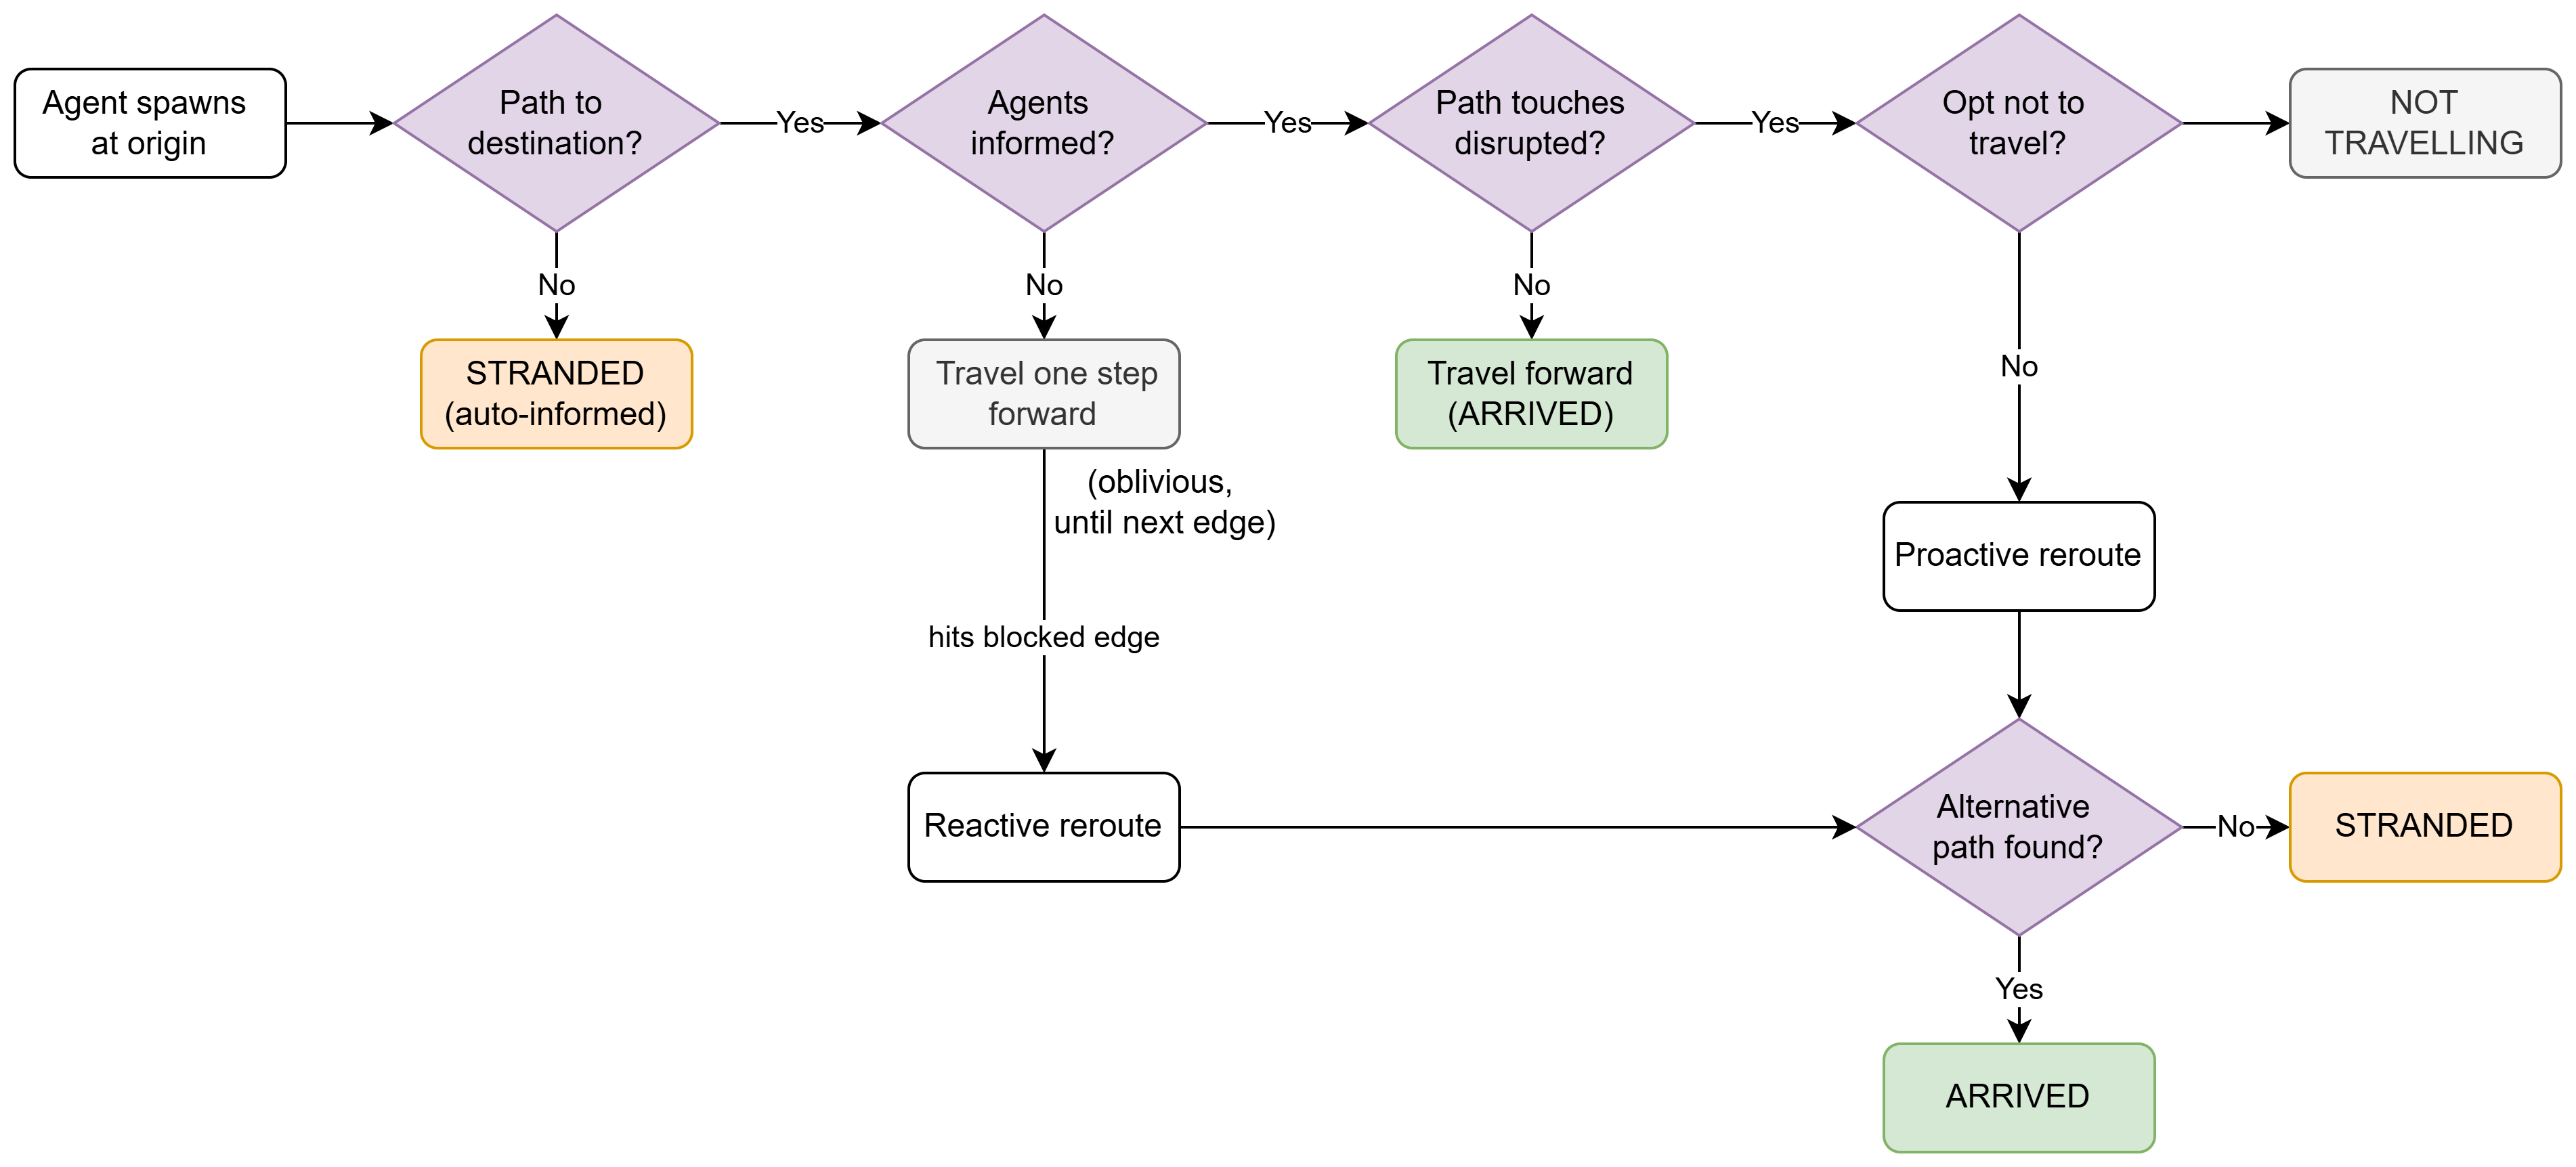
\includegraphics[width=0.95\linewidth]{Simulation_prj.png}
\caption{Agent decision logic per simulation step.}
\label{fig:mechanism}
\end{figure}

Three stylised stress-test scenarios are evaluated (Table~\ref{tab:scenarios}), each targeting a different network mechanism: hub closure, corridor disruption, and peripheral isolation.
Each scenario is static: following a 24-step warm-up of undisrupted travel, disruptions are applied at hour~24 and persist for the remaining 48~steps with no recovery, isolating the network-topology mechanism from temporal dynamics.

\begin{table}[h]
\centering
\caption{Disruption scenario specifications.}
\label{tab:scenarios}
\small
\resizebox{\linewidth}{!}{%
\begin{tabular}{llll}
\toprule
Scenario & Closed nodes & Closed corridors & Primary mechanism \\
\midrule
A: Northern Storm    & London, Amsterdam, Hamburg & --                          & Hub closure \\
B: Alpine Freeze     & Zurich                     & 28 Alpine rail edges         & Corridor disruption \\
C: Atlantic Cascade$^{\ast}$  & Lisbon, Porto              & Iberian rail + Paris CDG air & Peripheral isolation \\
\bottomrule
\end{tabular}}
\par\smallskip
{\footnotesize $^{\ast}$~CDG air connections to Iberia are disrupted alongside Iberian rail,
instantiating a spatially compounding event in the typology of \citet{Zscheischler2020}.}
\end{table}

\subsection{Information Layer}

Following \citet{Leng2020} and \citet{Cats2014}, an awareness layer tracks
whether each agent is informed of the disruption;
the approach builds on information-contagion models for transit disruptions
\citep{HuaOng2018}. Awareness spreads according to a Bass-type diffusion equation:
\begin{equation}
  \frac{\Delta I}{\Delta t} \;=\;
  \underbrace{p_{\text{int}}(t) \cdot S}_{\text{broadcast}} \;+\;
  \underbrace{q_{\text{contact}} \cdot \frac{I \cdot S}{N}}_{\text{peer contact}},
  \label{eq:si}
\end{equation}
where $I$ is the number of informed agents, $S = N - I$ the number of uninformed,
$N$ the total active agents, $p_{\text{int}}$ is the broadcast rate (mass media and app notifications),
$q_{\text{contact}}$ the peer-contact rate, and $I(0) = p_{\text{init}} \cdot N$ is the initial
informed share (agents already aware of the disruption at onset).
The contact term $q_{\text{contact}} \cdot IS/N$ is mean-field (modelling phone and social-media contact), not diffusion over a co-location network.
Two further channels operate outside Equation~\ref{eq:si}: an agent reaching a blocked edge discovers the disruption immediately (\emph{experiential}), and a topologically stranded agent is automatically informed (\emph{forced}).
All four channels are decomposed in Table~\ref{tab:pathways}.

%% =======================================================================
\section{Data and Calibration}
\label{sec:calibration}
%% =======================================================================

Calibration is inspired by the pattern-oriented modelling (POM) approach of \citet{Grimm2005}:
summary statistics from observed behaviour are matched across multiple patterns rather
than a single aggregate.

\subsection{Network Data}

\emph{Rail edges} are constructed from General Transit Feed Specification (GTFS) timetables of national operators of relevant countries.\footnote{GTFS feeds accessed April 2026:
  \href{https://www.gtfs.de/en/feeds/de_fv/}{DB};
  \href{https://transport.data.gouv.fr/datasets/horaires-sncf}{SNCF};
  \href{https://data.oebb.at/de/datensaetze~soll-fahrplan-gtfs~}{\"{O}BB};
  \href{https://nap.transportes.gob.es/Files/Detail/897}{Renfe};
  \href{https://archive.opentransportdata.swiss/timetable_gtfs_archive.htm}{SBB};
  \href{https://www.cciss.it/nap/mmtis/public/en/catalog/Asset/204135}{Trenitalia};
  \href{https://gtfs.ovapi.nl/nl/gtfs-nl.zip}{NS/OVapi};
  \href{https://data.belgianmobility.io/en/data.html}{SNCB};
  \href{https://www.transit.land/feeds/f-eyc-cp}{CP};
  \href{https://transport.data.gouv.fr/datasets/eurostar-gtfs-plan-de-transport-et-temps-reel}{Eurostar GTFS}, accessed 30~April~2026.}
A frequency cap of 20~trains/day restricts edges to intercity services; commuter routes
are excluded.
Routing uses Dijkstra on the time-weighted directed graph; service windows are 05:00--22:59 for air and day rail, 20:00--08:59 for night rail.

\emph{Air edges} are derived from Open Performance Data Initiative (OPDI) flight-list
data\footnote{\href{https://www.opdi.aero/flight-list-data}{OPDI flight-list data}, accessed 30 April 2026.}
(January~2022--March~2026).
Travel time equals haversine distance divided by 800~km/h \citep{ESPON2013} plus
a 45~min boarding overhead as a conservative modelling assumption informed by airport-process guidance \citep{IATA2023}.
\subsection{Gravity Demand Calibration}

OD volumes are estimated using structural gravity \citep{Anderson2003} with
Poisson Pseudo-Maximum-Likelihood (PPML; \citealt{SantosSilva2006}),
recently applied to German domestic and neighbouring-country rail-air substitution by \citet{Oesingmann2025}.
Separate models are fitted for air and rail (Table~\ref{tab:gravity}).

The \textbf{air model} includes origin and destination city fixed effects:
\begin{equation}
  V_{ij}^{\text{air}} = \exp\!\left(\alpha_i + \beta_j - \gamma_{\text{air}}
  \log d_{ij}\right).
  \label{eq:gravity_air}
\end{equation}

The \textbf{rail model} uses log travel time with symmetric population and a
same-country dummy (city fixed effects are excluded):\footnote{The rail OD set contains
134~pairs; including city fixed effects (FE) would require ${\approx}51$ FE parameters,
producing catastrophic overfit confirmed in preliminary runs.}
\begin{equation}
  V_{ij}^{\text{rail}} = \exp\!\left(\theta \log(P_i P_j)
  + \phi \left|\log P_i - \log P_j\right|
  - \gamma_{\text{rail}} \log t_{ij}
  + \delta \,\mathbf{1}[\text{same country}]\right).
  \label{eq:gravity_rail}
\end{equation}

The GTFS proxy measures supply frequency rather than observed OD demand, a limitation
inherent to network-scale European rail modelling at this geographic scope; the
level~$R^2$ reflects structural noise in the proxy rather than a failure of the gravity
specification.
The ABM uses demand weights for stochastic OD sampling, not for point prediction of
passenger counts: rank order of pairs determines which corridors attract most agents,
and the Spearman correlation of 0.611 (Table~\ref{tab:gravity}) confirms this ordering is
preserved in the test set, supporting its use for coarse demand-weighted OD sampling.
Route-specific modal split:
\begin{equation}
  s_{ij}^{\text{air}} = \frac{V_{ij}^{\text{air}}}{V_{ij}^{\text{air}} + V_{ij}^{\text{rail}}}.
  \label{eq:modal_split}
\end{equation}
Because $V_{ij}^{\text{rail}}$ is derived from GTFS service frequency (a supply proxy)
rather than observed OD passenger counts, this ratio should be interpreted as a
calibrated supply-weighted routing prior rather than an empirically observed modal share.
The OD sampling weight used by the ABM is:
\begin{equation}
  w_{ij} = s_{ij}^{\text{air}} \cdot V_{ij}^{\text{air}} \;+\;
            (1 - s_{ij}^{\text{air}}) \cdot V_{ij}^{\text{rail}}.
  \label{eq:od_weight}
\end{equation}

\begin{table}[h]
\centering
\caption{Gravity calibration results: v4 dual-mode model.}
\label{tab:gravity}
\small
\begin{tabular}{lllccc}
\toprule
Mode & Estimator & Specification & $\hat{\gamma}$ & $R^2$ (test) & Spearman $\rho$ \\
\midrule
Air  & PPML + city FE & log-distance
     & 0.189 & 0.610 & 0.793 \\
Rail & PPML, no FE    & log-travel-time + sym-pop + same-country
     & 0.422 & 0.333 & 0.611 \\
\bottomrule
\end{tabular}
\end{table}

\subsection{Behavioural Prior Calibration and Event-Level Plausibility Check}
\label{sec:layer_e}

\emph{Information diffusion.}
Because no transport-specific estimates exist for hourly information acquisition during a pan-European multimodal disruption, $p_{\text{int}}$ and $q_{\text{contact}}$ are treated as behavioural scenario parameters rather than fitted coefficients.
The values $p_{\text{int}} = 0.30$~h$^{-1}$ and $q_{\text{contact}} = 0.20$~h$^{-1}$ are set so that broadcast dominates peer contact, consistent with \citet{ORRAECOM2017}; these parameters govern the timing of awareness, not the topology of feasible paths, and should be interpreted as stress-test assumptions rather than calibrated behavioural estimates.
An initial informed share of 0.05 is a conservative assumption for sudden-onset disruption.\footnote{\citet{DArienzo2020} and \citet{OShea2020} motivate the two-channel warning structure but are not used numerically, as their empirical settings differ from disrupted transport. At $p_{\text{int}} = 0.30$~h$^{-1}$, independent broadcast awareness reaches approximately 66\% after three hours and 88\% after six hours (discrete per-step formula); the grid upper bound $p_{\text{int}} = 0.50$~h$^{-1}$ implies approximately 98\%, representing a near-instantaneous scenario. \citet{ORRAECOM2017} reports high pre-travel awareness for \emph{planned} disruptions (74--76\%) and is used here only as a behavioural reference for channel ranking and rescheduling response, not as direct calibration for sudden-onset awareness.}

\emph{Disruption response.}
The probability that an informed agent opts not to travel, $p_{\text{reschedule}} = 0.13$: consistent with the 13\%
`choose not to travel' rate observed among non-London long-distance rail passengers
facing service disruption \citep[Table~3.4]{ORRAECOM2017}.
Rerouting interval $r = 4$~h: a modelling assumption representing a realistic re-planning
cycle for an informed agent mid-journey; in full-node-closure scenarios the daytime service
window overrides this interval, making stranding geography analytically insensitive to its exact value.

\emph{Event-level plausibility check against Storm Ciaran.}
The stranding geography produced by the network and demand layers is compared against
Storm Ciaran (1--2~November~2023) as an event-level plausibility check.
The information parameters ($p_{\text{int}}$, $q_{\text{contact}}$) are not validated here:
they govern awareness timing, not which cities strand, and stranding is topology-determined.
OPDI disruption severity per city (fractional flight reduction vs.\ a same-weekday baseline)
correlates positively with ABM-simulated stranding counts across 34 cities
($\rho = 0.498$, $p = 0.003$; Figure~\ref{fig:ciaran}), supporting external plausibility.
This should be interpreted as an event-level plausibility check rather than full predictive
validation, as the same OPDI dataset underlies both air network construction and the severity measure.

\begin{figure}[h]
\centering

\includegraphics[width=0.55\textwidth]{figures/ciaran_validation_scatter.pdf}
\caption{Storm Ciaran event-level plausibility check ($\rho = 0.498$, $p = 0.003$, $n = 34$).
         $x$-axis: OPDI disruption severity (fractional flight reduction vs.\ baseline).
         $y$-axis: ABM-simulated mean stranded agents.}
\label{fig:ciaran}
\end{figure}


%% =======================================================================
\section{Results}
\label{sec:results}
%% =======================================================================

\subsection{Baseline Connectivity Check}

Zero agents strand across all five Monte Carlo baseline runs ($\sigma_c = 0$ for all cities),
confirming that all sampled OD pairs remain routable under normal service.

\begin{figure}[h]
\centering

\includegraphics[width=\textwidth]{figures/scenario_dynamics.pdf}
\caption{\textit{Top}: per-hour arrivals and strandings (mean $\pm$~SD, 5~runs);
         dashed line at hour~24 marks disruption onset; overnight dips reflect service-window
         closure (23:00--05:00). \textit{Bottom}: stranding geography.}
\label{fig:dynamics}
\end{figure}

\subsection{Scenario Outcomes}
\textbf{Scenario A: Northern Storm.}
Closing London, Amsterdam, and Hamburg produces the highest total stranding burden across all three scenarios.
The most striking pattern is \emph{secondary stranding}: hinterland cities (Essen, Dortmund)
outrank closed hubs because they depend on Amsterdam or Hamburg for nearly all intercity connections,
illustrating the interdependency regime of \citet{Buldyrev2010}.
Stranding stabilises within hours of onset: information diffusion affects timing but not the
final stranded count, as the binding constraint is topological.

\textbf{Scenario B: Alpine Freeze.}
Total stranded passengers are substantially lower than in Scenario~A
because air alternatives from Milan, Vienna, and Geneva remain operational.
Zurich is the sole focus of stranding (Table~\ref{tab:stranding});
the second-highest city, Palermo, has a stranding index almost seven times lower,
illustrating the focused nature of the Alpine disruption.
This produces the engineering/ecological resilience contrast of \citet{Reggiani2015}:
Zurich exhibits hard engineering failure (stranding), while neighbouring cities show elevated delay only.
Informed agents successfully reroute around partial Alpine blockages, suggesting that awareness improves outcomes where alternatives exist \citep{Leng2020}.

\textbf{Scenario C: Atlantic Cascade.}
The Atlantic Cascade produces the broadest secondary stranding footprint (Table~\ref{tab:stranding}).
Travellers associated with Bilbao and Murcia have the highest stranding exposure
despite those cities not being directly closed
(Table~\ref{tab:stranding}): both depend entirely on rail-air corridors through Madrid or
Iberian coastal routes severed by the cascade.
Bilbao's index should be interpreted cautiously: it has no air OD pairs in the gravity
model due to OPDI transponder coverage gaps (Section~\ref{sec:conclusions}),
so its isolation partly reflects absent air alternatives in the data rather than the city's true connectivity.
Lisbon's position is critical: with no direct long-distance rail alternative to Spain in the modelled network, node closure severs every access path.
Madrid's 

\noindent
\begin{minipage}[t]{0.50\textwidth}
\captionof{table}{Top origin/destination exposure cities by stranding index.
         Hinterland cities without direct closure consistently outrank closed hubs.}
\label{tab:stranding}
\vspace{2pt}
\small
\begin{tabular}{lrrl}
\toprule
City & $\sigma_c$ & Raw count & Type \\
\midrule
\multicolumn{4}{l}{\textit{Scenario A: Northern Storm}} \\
Essen          & 0.339 &  52 & Hinterland \\
Brussels       & 0.332 &  98 & Hinterland \\
Bremen         & 0.332 &  33 & Hinterland \\
London         & 0.331 & 235 & Closed hub \\
Dortmund       & 0.330 &  61 & Hinterland \\
Hamburg        & 0.327 &  94 & Closed hub \\
Amsterdam      & 0.322 & 142 & Closed hub \\
\midrule
\multicolumn{4}{l}{\textit{Scenario B: Alpine Freeze}} \\
Zurich         & 0.319 &  92 & Closed hub \\
Palermo        & 0.047 &   2 & Hinterland \\
Strasbourg     & 0.036 &   6 & Hinterland \\
\midrule
\multicolumn{4}{l}{\textit{Scenario C: Atlantic Cascade}} \\
Bilbao         & 0.364 &  12 & Hinterland \\
Murcia         & 0.357 &  11 & Hinterland \\
Madrid         & 0.332 & 175 & Hinterland \\
Seville        & 0.329 &  39 & Hinterland \\
Porto          & 0.325 &  40 & Closed hub \\
Lisbon         & 0.322 &  85 & Closed hub \\
\bottomrule
\end{tabular}
\end{minipage}
\hfill
\begin{minipage}[t]{0.46\textwidth}
\centering
\captionof{figure}{Cumulative stranded vs.\ arrived-while-informed over 72~h by scenario.
         In Scenario~B informed arrivals exceed strandings; in A and~C stranding dominates,
         supporting the interpretation that awareness helps mainly where alternatives exist.}
\label{fig:si}
\vspace{2pt}

\includegraphics[width=\linewidth]{figures/si_diffusion.pdf}
\end{minipage}

disrupted air corridors propagate isolation across the south; the spatial compounding
\citep{Zscheischler2020} is evident across the geographic arc from Lisbon to Paris.

\subsection{Information-Layer Dynamics}

Figure~\ref{fig:si} supports the interpretation that information improves ecological resilience (Scenario~B, where alternatives exist) but cannot create engineering resilience where none exists \citep{Reggiani2015, Leng2020, Cats2014}.

\begin{table}[h]
\centering
\caption{Information-pathway summary per scenario (mean across 5~MC~runs, step~72).
         ``External'' denotes broadcast/app/official information;
         ``Peer'' denotes mean-field contact transmission;
         ``Experiential'' denotes blocked-edge or forced discovery after disruption exposure.}
\label{tab:pathways}
\small
\begin{tabular}{lccccc}
\toprule
Scenario & External \% & Peer \% & Experiential \% & Arrived-informed & Stranded \\
\midrule
A: Northern Storm   & 17.3 & 0.5 & 82.1 & 225 & 1481 \\
B: Alpine Freeze    & 54.9 & 6.1 & 39.0 & 522 &  191 \\
C: Atlantic Cascade & 35.1 & 3.1 & 61.8 & 345 &  662 \\
\bottomrule
\end{tabular}
\end{table}

Peer contact is a minor channel; broadcast dominates in Scenario~B, where partial disruption extends the proactive window \citep{Leng2020}.
In Scenarios~A and~C, experiential discovery accounts for over 60\% of awareness events, reflecting the sudden compound onset that leaves little proactive broadcast window.


\subsection{Centrality and Stranding Correlation}

Betweenness centrality shows moderate positive correlation with stranding in Scenario~A ($r = 0.418$), where the disrupted nodes are themselves the highest-centrality cities.
The relationship is weak in Scenarios~B ($r = 0.048$) and~C ($r = 0.185$), where stranding is driven by geographic proximity to the disruption arc rather than network position.
Direct exposure therefore dominates hard stranding; centrality amplifies secondary rerouting burden only when the disrupted nodes are major hubs.

\subsection{Sensitivity and Parametric Robustness}

Spawn-rate sensitivity ($\lambda \in \{100\text{--}1000\}$~h$^{-1}$) confirms stranding rates $\sigma_c$ are stable across a tenfold agent-population range.
Disruption probability sensitivity ($p_{\text{disrupt}} \in [0.5, 1.0]$) preserves city rank ordering; Scenario~C shows a threshold effect near full closure where the last Iberian paths fail simultaneously.
Air-overhead sensitivity (45, 90, and 120~min boarding assumptions) produces
identical top-stranded city rankings across all scenarios and changes total stranding
by less than 3\% (Scenario~C: 662 to 678); shortest-path routing and modal split
are robust to the overhead parameterisation.
Information-parameter sensitivity across 16 combinations ($p_{\text{int}} \in \{0.10,0.20,0.30,0.50\}$~h$^{-1}$, $q_{\text{contact}} \in \{0.05,0.10,0.20,0.40\}$~h$^{-1}$) spans a range from slow diffusion to near-instantaneous broadcast awareness (the upper bound $p_{\text{int}} = 0.50$~h$^{-1}$ implies approximately 98\% independent awareness within six hours): Scenario~B arrived-informed exceeds A and~C in all 16 combinations, stranding deviates by at most 1\% (A) and 2\% (C), and top-ranked cities are identical across the full grid, confirming that topology dominates awareness in Scenarios~A and~C.

\textbf{Compound ablation.}
To isolate the interdependency contribution, each scenario was re-run under
rail-only and air-only disruption with scenario geometry held constant
(Table~\ref{tab:ablation}).
In Scenarios~B and~C neither single mode alone produces stranding: compound disruption
uniquely removes both modal alternatives simultaneously.
In Scenario~A, rail-only disruption produces just 21\% of the compound total,
confirming that simultaneous air and rail closure drives most stranding.
These results align with the \citet{Buldyrev2010} interdependency mechanism.

\begin{table}[h]
\centering
\caption{Compound ablation: total stranded agents by disruption mode.}
\label{tab:ablation}
\small
\begin{tabular}{lccc}
\toprule
Scenario & Compound & Rail-only & Air-only \\
\midrule
A: Northern Storm   & 1,481 & 310 & 0 \\
B: Alpine Freeze    &   191 &   0 & 0 \\
C: Atlantic Cascade &   662 &   0 & 0 \\
\bottomrule
\end{tabular}
\end{table}

%% =======================================================================
\section{Conclusions}
\label{sec:conclusions}
%% =======================================================================

This paper simulated passenger redistribution across a 53-city European multimodal
transport network under three compound weather-disruption scenarios, compared against
Storm Ciaran as an external plausibility check.
Three main findings emerge.

First, \emph{topology is the binding constraint on hard stranding}.
Direct node closures produce stranding that information diffusion cannot overcome:
when no path exists, awareness of that fact does not create one.
A compound ablation supports the interdependency mechanism described by \citet{Buldyrev2010}:
single-mode disruption alone produces little or no stranding across scenarios,
while compound disruption produces substantially more, underlining that simultaneous
multi-modal failure is qualitatively distinct from either mode failing in isolation.

Second, \emph{peripheral air-dependent cities are the most vulnerable}.
Lisbon, with no direct long-distance rail alternative to Spain in the modelled network,
becomes a topological island under node closure.
Bilbao and Murcia, though not directly closed, record the highest stranding indices
in Scenario~C (Table~\ref{tab:stranding}) because all their connections route through
disrupted corridors; Bilbao's exact value should be interpreted cautiously given missing
air OD coverage (see Limitations), but Murcia's ranking is unaffected by that gap.
The results suggest that compound weather risk is not uniformly distributed but
concentrates at cities with structurally limited multimodal alternatives, a pattern
with direct implications for network resilience planning by bodies such as ERA and EUROCONTROL.

Third, \emph{information timing matters only where alternatives exist}.
The awareness layer has measurable effects in Scenario~B, where partial connectivity survives,
but negligible effects in Scenarios~A and~C.
Information improves ecological resilience only where alternatives survive; where topology
removes all paths, awareness cannot prevent hard stranding \citep{Reggiani2015};
this result is invariant to broadcast and peer-contact rate variation (Section~\ref{sec:results}).

\textbf{Limitations.}
The model captures topological isolation under static disruptions, not congestion on surviving routes or recovery dynamics; each city is a single node and demand is gravity-modelled rather than from observed origin-destination matrices.
OPDI covers only actual ADS-B departures, so delay-dominated events produce attenuated validation signals, and coverage gaps leave Bilbao and three other cities with missing air OD pairs, so Bilbao's stranding index partly reflects absent data rather than pure network topology.
Sensitivity sweeps for $p_{\text{init}}$ and $p_{\text{reschedule}}$ were not performed; as these affect awareness timing rather than path existence, they are unlikely to alter city rankings, but this remains a limitation.

\textbf{Future work.}
Priority extensions include temporal recovery dynamics, capacity-constrained rerouting on
surviving corridors, and probabilistic disruption-intensity sweeps.
Pre-planned agent types (departures hours away when the warning arrives) would isolate the causal effect of early information on stranding outcomes.

%% =======================================================================
%%  REFERENCES  (excluded from 10-page limit per course instructions)
%% =======================================================================

\begin{thebibliography}{99}

\bibitem[AECOM(2017)ORRAECOM2017]{ORRAECOM2017}
AECOM (2017).
\textit{Research into Passengers' Awareness of Planned Disruption.
Final Study Report Version~2}.
Prepared for the Office of Rail and Road (ORR).
Available: \url{https://www.orr.gov.uk/sites/default/files/om/aecom-report-research-into-passengers-awareness-of-planned-disruption.pdf}
[Accessed: 30 May 2026].

\bibitem[Anderson and van~Wincoop(2003)Anderson2003]{Anderson2003}
Anderson, J.~E. and van~Wincoop, E. (2003).
Gravity with gravitas: a solution to the border puzzle.
\textit{American Economic Review}, 93(1):170--192.

\bibitem[Bass(1969)Bass1969]{Bass1969}
Bass, F.~M. (1969).
A new product growth model for consumer durables.
\textit{Management Science}, 15(5):215--227.

\bibitem[Berdica(2002)Berdica2002]{Berdica2002}
Berdica, K. (2002).
An introduction to road vulnerability: what has been done, is done and should be done.
\textit{Transport Policy}, 9(2):117--127.


\bibitem[Buldyrev et~al.(2010)Buldyrev2010]{Buldyrev2010}
Buldyrev, S.~V., Parshani, R., Paul, G., Stanley, H.~E., and Havlin, S. (2010).
Catastrophic cascade of failures in interdependent networks.
\textit{Nature}, 464:1025--1028.

\bibitem[Cats and Jenelius(2014)Cats2014]{Cats2014}
Cats, O. and Jenelius, E. (2014).
Dynamic vulnerability analysis of public transport networks: mitigation effects of
real-time information.
\textit{Networks and Spatial Economics}, 14:435--463.

\bibitem[D'Arienzo et~al.(2020)DArienzo2020]{DArienzo2020}
D'Arienzo, M., Di~Paolo, F., Chiacchiararelli, L., Malizia, A., and Indovina, L. (2020).
A mathematical model for the diffusion of emergency warning messages during {CBRNe} emergencies.
\textit{Journal of Contingencies and Crisis Management}, 28(3):228--239.

\bibitem[Epstein and Axtell(1996)Epstein1996]{Epstein1996}
Epstein, J.~M. and Axtell, R. (1996).
\textit{Growing Artificial Societies: Social Science from the Bottom Up}.
MIT Press, Cambridge, MA.

\bibitem[ESPON(2013)ESPON2013]{ESPON2013}
ESPON (2013).
\textit{{TRACC}: Transport Accessibility at Regional/Local Scale and Patterns in Europe}.
Applied Research Project 2013/1/7.
ESPON Coordination Unit, Luxembourg.

\bibitem[Grimm et~al.(2005)Grimm2005]{Grimm2005}
Grimm, V., Revilla, E., Berger, U., Jeltsch, F., Mooij, W.~M., Railsback, S.~F.,
et~al.\ (2005).
Pattern-oriented modeling of agent-based complex systems: lessons from ecology.
\textit{Science}, 310(5750):987--991.

\bibitem[Grimm et~al.(2020)Grimm2020]{Grimm2020}
Grimm, V., Railsback, S.~F., Vincenot, C.~E., Berger, U., Gallagher, C.,
DeAngelis, D.~L., et~al.\ (2020).
The ODD protocol for describing agent-based and other simulation models: a second update.
\textit{Journal of Artificial Societies and Social Simulation}, 23(2):7.

\bibitem[Holling(1973)Holling1973]{Holling1973}
Holling, C.~S. (1973).
Resilience and stability of ecological systems.
\textit{Annual Review of Ecology and Systematics}, 4:1--23.

\bibitem[Hua and Ong(2018)HuaOng2018]{HuaOng2018}
Hua, W. and Ong, G.~P. (2018).
Effect of information contagion during train service disruption for an integrated
rail-bus transit system.
\textit{Public Transport}, 10:571--594.

\bibitem[IATA(2019)IATA2023]{IATA2023}
IATA (2019).
\textit{Airport Development Reference Manual}, 11th~edn.
International Air Transport Association, Montreal.

\bibitem[IPCC(2023)IPCC2023]{IPCC2023}
IPCC (2023).
\textit{Climate Change 2023: Synthesis Report}.
Contribution of Working Groups I, II and III to the Sixth Assessment Report.
IPCC, Geneva.

\bibitem[Ippolito and Cats(2024)Ippolito2024]{Ippolito2024}
Ippolito, D. and Cats, O. (2024).
Multi-modal and multi-layer robustness analysis of the European rail and air networks.
\textit{Scientific Reports}, 14:26950.

\bibitem[Jenelius et~al.(2006)Jenelius2006]{Jenelius2006}
Jenelius, E., Petersen, T., and Mattsson, L.-G. (2006).
Importance and exposure in road network vulnerability analysis.
\textit{Transportation Research Part A}, 40(7):537--560.

\bibitem[Leng and Corman(2020)Leng2020]{Leng2020}
Leng, N. and Corman, F. (2020).
The role of information availability to passengers in public transport disruptions:
an agent-based simulation approach.
\textit{Transportation Research Part A}, 133:214--236.

\bibitem[Little(1961)Little1961]{Little1961}
Little, J.~D.~C. (1961).
A proof for the queuing formula: {$L = \lambda W$}.
\textit{Operations Research}, 9(3):383--387.

\bibitem[Mattsson and Jenelius(2015)Mattsson2015]{Mattsson2015}
Mattsson, L.-G. and Jenelius, E. (2015).
Vulnerability and resilience of transport systems: a discussion of recent research.
\textit{Transportation Research Part A}, 81:16--34.

\bibitem[Oesingmann and Ennen(2025)Oesingmann2025]{Oesingmann2025}
Oesingmann, K. and Ennen, D. (2025).
The impacts of high-speed rail expansion on short-haul air passenger transport:
evidence from German domestic and international traffic.
\textit{Case Studies on Transport Policy}, 21:101549.

\bibitem[O'Shea et~al.(2020)OShea2020]{OShea2020}
O'Shea, T., Bates, P., and Neal, J. (2020).
Testing the impact of direct and indirect flood warnings on population behaviour
using an agent-based model.
\textit{Natural Hazards and Earth System Sciences}, 20:2281--2305.

\bibitem[Reggiani et~al.(2015)Reggiani2015]{Reggiani2015}
Reggiani, A., Nijkamp, P., and Lanzi, D. (2015).
Transport resilience and vulnerability: the role of connectivity.
\textit{Transportation Research Part A}, 81:4--15.

\bibitem[Santos~Silva and Tenreyro(2006)SantosSilva2006]{SantosSilva2006}
Santos~Silva, J.~M.~C. and Tenreyro, S. (2006).
The log of gravity.
\textit{Review of Economics and Statistics}, 88(4):641--658.

\bibitem[Zscheischler et~al.(2020)Zscheischler2020]{Zscheischler2020}
Zscheischler, J., Martius, O., Westra, S., Bevacqua, E., Raymond, C.,
Horton, R.~M., et~al.\ (2020).
A typology of compound weather and climate events.
\textit{Nature Reviews Earth \& Environment}, 1:333--347.

\end{thebibliography}

\end{document}
